\documentclass[10pt,psamsfonts]{amsart}

%-------Packages---------
\usepackage{amssymb,amsfonts}
%\usepackage[all,arc]{xy}
\usepackage{enumerate}
%\usepackage{mathrsfs}
\usepackage{subcaption}
\usepackage{graphicx}
\usepackage{caption}
\usepackage[margin=1in]{geometry}
\usepackage{tabularx}

%--------Theorem Environments--------
%theoremstyle{plain} --- default
\newtheorem{thm}{Theorem}[section]
\newtheorem{cor}[thm]{Corollary}
\newtheorem{prop}[thm]{Proposition}
\newtheorem{lem}[thm]{Lemma}
\newtheorem{conj}[thm]{Conjecture}
\newtheorem{quest}[thm]{Question}

\theoremstyle{definition}
\newtheorem{defn}[thm]{Definition}
\newtheorem{defns}[thm]{Definitions}
\newtheorem{con}[thm]{Construction}
\newtheorem{exmp}[thm]{Example}
\newtheorem{exmps}[thm]{Examples}
\newtheorem{notn}[thm]{Notation}
\newtheorem{notns}[thm]{Notations}
\newtheorem{addm}[thm]{Addendum}
\newtheorem{exer}[thm]{Exercise}

\theoremstyle{remark}
\newtheorem{rem}[thm]{Remark}
\newtheorem{rems}[thm]{Remarks}
\newtheorem{warn}[thm]{Warning}
\newtheorem{sch}[thm]{Scholium}

\newcommand\setrow[1]{\gdef\rowmac{#1}#1\ignorespaces}
\newcommand\clearrow{\global\let\rowmac\relax}

\makeatletter
\let\c@equation\c@thm
\makeatother
\numberwithin{equation}{section}

\bibliographystyle{plain}

%--------Meta Data: Fill in your info------
\title{Automated Essay Grading from Scratch}

\author{Won I. Lee, Qin Lyu, and Zelong Qiu}

%\date{July 30, 2016}

\begin{document}
	
\maketitle

\begin{abstract}
	Automated essay grading is an important problem for advancing curricular assessments in K-12 education, as it allows for rapid evaluation of student-constructed responses and opens the way for the assessment of more sophisticated analytical and reasoning skills.  In this work, we investigate the performance of various deep architectures on the task of automated essay grading. We employ no hand-crafted features and explore both character-level and word-level models for this task, using both convolutional and recurrent architectures. We find that these different architectures and training paradigms offer complementary advantages on this task. In addition, we provide a more nuanced analysis of the strengths of various architectural and training choices by considering performance across a variety of metrics, showing that while certain models performed better on raw classification accuracy, others predicted scores that were closer on average to the actual scores.
\end{abstract}

\section*{Introduction and Related Work}

One prominent impediment preventing the enhancement of curricula in K-12 education to focus more on critical reasoning ability and analytical skills is the difficulty of scoring tests to measure these abilities. It is generally the case that measuring such skills requires inviting the student for open-ended answers rather than simple, multiple-choice ones; unfortunately, tests that require essays or other individually-written responses are difficult to score automatically and necessitate scoring by human graders. Such grading involves substantial time and expense from both testing companies and government agencies (for standardized exams), and as a result, most such tests have relied more on multiple-choice questions, limiting the ability to assess more sophisticated skills.

This has long motivated the development of automated system for essay grading. Much effort has been put into building a satisfactory system that could reliable generate scores in line with those of human judges. The Intelligent Essay Assessor (IEA) was first used to score essays for large undergraduate courses in 1994 \cite{iea}, and the e-Rater, an automated reader developed by the Educational Testing Service was used to grade large-scale essays on standardized exams \cite{erater}.

All of these examples used on the order of hundreds of hand-crafted features to generate the essay scores. Recently, however, the development of more automatic methods in natural language processing based on deep neural networks has suggested that systems for such tasks boasting comparable or even superior performance can be constructed ``from scratch'' without manually crafting features for the algorithm. For example, the work of Collobert et al. \cite{collobert}, which helped to inspire the current wave of deep learning applications in NLP, demonstrated that appropriately-trained neural network models incorporating no hand-crafted features could achieve performance rivaling that of state-of-the-art systems based on extensive feature crafting.

More recently, a variety of deep architectures have emerged for various tasks in NLP. In particular, the sequence-to-sequence model, incorporating two LSTMs (encoder and decoder), has emerged as the paradigm for sequential tasks such as machine translation \cite{s2s}. Certain architectures often consider character-level inputs instead of or in addition to word-level inputs, often employing convolutional neural networks (CNNs) as a representation-generating layer before feeding into a fully-connected model or recurrent network \cite{lecun}.

All of these networks offer important features and benefits that are suitable for certain tasks. For the task of automated essay grading, however, we note that many of the advantages offered by each respective model are desirable. For example, as described below, it would be beneficial to employ character-level inputs for essay grading; in another vein, the sequential information captured by recurrent networks are often vital to judging the quality of essays. Thus, in this work, we report on a series of experiments testing which model architectures work best for the task of automated essay grading. Of course, we cannot be exhaustive in this search, but we aim to provide an illustrative and meaningful look at the advantages of certain architectures and training methods over others.

\section*{Data}

Our dataset consists of essays selected from 8 different essay prompts across a variety of exams. These essay sets differ in the length of essays with which they are associated, their possible score ranges, and the number of examples, among other qualities. We provide an illustration of the statistics associated with each essay set in Table \ref{fig:data}, demonstrating the large variability in the score ranges and number of examples.

The dataset contains both the essay set ID and essay ID, as well as the entire text of the essay. For evaluation, the dataset contains one or more human scores, and the final resolved human score (generally an average of scores if there are multiple available for a given essay). The final resolved score is the measure of interest for this task, and in our experiments we only consider this measure as the quantity of interest.

\begin{table}
	\begin{tabular}{c|c|c|c|c}
		Essay Set & Score Range & Train Set Size & Valid Set Size & Test Set Size\\\hline
		1 & 2-12 & 1426 & 179 & 178\\
		2 & 1-6 & 1416 & 193 & 191\\
		3 & 0-3 & 1384 & 166 & 176\\
		4 & 0-3 & 1407 & 183 & 180 \\
		5 & 0-4 & 1458 & 178 & 169\\
		6 & 0-4 & 1458 & 157 & 185\\
		7 & 0-30 & 1257 & 151 & 161\\ 
		8 & 0-60 & 612 & 52 & 59\\\hline
		Total & 0-60 & 10419 & 1260 & 1300
	\end{tabular}
	\caption{Statistics for the data set of essays and scores.}
	\label{fig:data}
\end{table}

\section*{Models}

\subsection*{Character-Level CNN}\hfill\\
\vskip -0.1in

A prominent issue with essay grading is that many of the words in candidate essays are misspelled, so that they lie outside a fixed vocabulary. Most models with fixed vocabulary word embeddings can only deal with such words by treating them as ``UNK'' tokens, which removes any information that such words may convey about the quality of the essay. Unlike most natural language tasks for which out-of-vocabulary words are infrequent and often unimportant, misspellings can provide valuable information regarding the quality of the writing for grading student essays.

One way to deal with such cases is to consider character-level models rather than word-level models. Thus, we consider a character-level convolutional neural network (CNN), which embeds each character into a $d$-dimensional vector ($d \approx 30$) and employs a series of 1D convolutions and max-pooling layers to extract efficient representations for inference. We stack fully-connected layers on top of the convolutional layers for final processing, and use either dense or one-hot encodings of the characters as input. We provide a schematic of our overall architecture in Figure \ref{fig:cnn}. We consider a 6 convolutional layer model inspired by the work of Zhang, Zhao, and LeCun, 2015 \cite{charnn} as well as a simpler, 1 convolutional layer model inspired by the work of Kim, 2014 \cite{kim14}.

\begin{figure}
	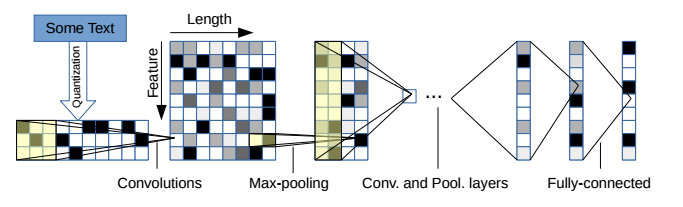
\includegraphics[width=\textwidth]{cnn.png}
	\caption{Architecture of character-level CNN model; figure credit to Zhang, X., J. Zhao, and Y. LeCun (2015).}
	\label{fig:cnn}
\end{figure}

{\em Training.} In this formulation, we primarily treated the essay score as a percentage of the score range (i.e. for essay set 1, which has range 2-12, an essay with score 6 would be treated as 0.4), and used logistic regression as our final output. We used standard stochastic gradient descent (SGD) with momentum for training, using binary cross-entropy loss as our objective.

\subsection*{Word-Level Deep Neural Network}\hfill\\
\vskip -0.1in

An issue encountered in character-level models on this task, however, is that the models are unable to leverage the semantic information of words in order to make better predictions regarding essay quality. The word-level DNN model was built to model each essay as an ``averaged word''. The logic behind this idea is that the usage of certain words over others could represent the quality of an essay. There could be more sophisticated or ``good'' words that the essays with high scores tend to contain, and similarly common or ``bad'' words that are usually associated with low-quality essays. In addition, since all misspelled words are given zero vectors (as they lie outside the vocabulary), this model could easily discriminate essays with a lot of misspelled words, which have an average value near 0, from those containing few misspelled words. 

In the data processing stage, the pretrained GLoVe word vectors are utilized to embed all the word in an essay to a fixed length, and these embeddings are then averaged to get the ``average word vector'' of an essay. These fixed dimension ``average word vectors'' are then fed into a fully-connected deep neural network model with 5 hidden layers and rectifier linear unit (ReLU) activation. We consider two different types of output layers, corresponding to different problem formulations. Treating scores as a classification problem, we employ a softmax layer for the output, using 61 units representing all the possible scores ranging from 0 to 60. On the other hand, we can treat scores as a regression problem, for which the output layer is one single unit with linear activation for prediction of a real number value (also known as a multilayer perceptron (MLP) model). The architecture is shown in Figure \ref{fig:dnn}.

{\em Training.} In the training stage, we used either categorical cross-entropy (for classification) or squared-error (for regression) as our loss criteria. Training naively yielded two over-fitted models for DNN classification and MLP. Then, the models were regularized by introducing elastic net regularization and dropout at each layer. The best-performing model was obtained by using the ``checkpoint'' functionality in Keras package to record the best performance over validation set, essentially using a form of early stopping.

A limitation of these models is that they only consider the wording of an essay without taking the ordering of words, sentence structures, and essay length into consideration. In fact, an essay with proper wording and perfect sentence structure will be embedded exactly same as an essay with the same words but completely disordered sentence structure. 

\begin{figure}
	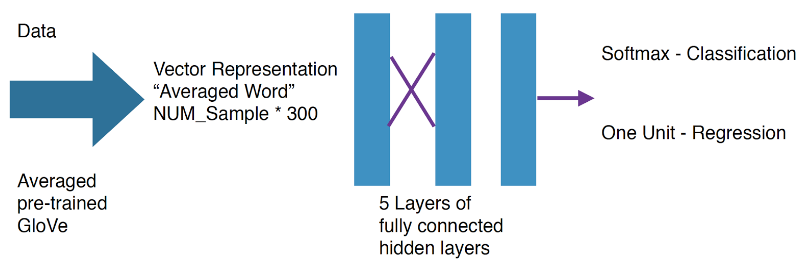
\includegraphics[width=0.6\textwidth]{dnn.png}
	\caption{Architecture of ``average-word'' fully-connected deep NN.}
	\label{fig:dnn}
\end{figure}

\subsection*{Sentence-Level LSTM and Pairwise Ranking Model}\hfill\\
\vskip -0.1in

To rectify the above problem, we also consider sentence-level models for essay grading. Suppose each sentence is encoded into a vector of fixed dimension; then the essay can be seen as a series of sentence vectors. Hence it is natural to use an LSTM model to capture sentence-level transition patterns in each essay and measure the quality of essays by assessing such patterns. There are two ways to encode a sentence into a vector:
\begin{enumerate}
\item Bag-of-Words model: The sentence vector is the sum of word vectors of the words in the sentence.
\item Sequence model: The sentence vector is the output of another LSTM model, whose input is the word vector sequence of the words in the sentence. 
\end{enumerate}
To reduce computational complexity, we use the bag-of-words model to encode each sentence into a vector, where the pretrained word vectors are provided by GloVe \cite{glove}.

One issue encountered in the classification and regression models in this task is that the score range is different across sets. In the previous section, we addreseds this issue by normalizing the score to real values in $[0, 1]$. However, essays from different set may not be comparable as the assessment standard is different from one set to another. Both the classification and regression models are trained with essays from all 8 sets with absolute scores, which implicitly introduces incorrect order information. Hence we consider using a ranking model to learn the score order instead of learning the scores directly. 

{\em Training.} We consider pairs of essays from the same essay set. For each pair $(d_l, d_r)$, we assign label 0 if $score_l>score_r$ and label 1 if $score_l<score_r$. In other words, labels represent the order information of essay pairs. Denote by $o_i$ the output score of sentence-level LSTM model with input essay $d_i$. We then use the cross entropy loss function:
$$L_{ij}\equiv L(o_{ij})=-y_{ij}\log P_{ij}-(1-y_{ij})\log(1-P_{ij})$$ 
where $o_{ij}\equiv o_i-o_j, P_{ij}\equiv 1/(1+e^{-o_{ij}})$, and $y_{ij}$ is the label of $(d_i, d_j)$. In fact, this is the pairwise loss function proposed by Burges et al., 2005 \cite{ranknet}.

The model architecture is shown in Figure \ref{fig:rankmodel}. Note that we add one more LSTM layer in the reverse direction to further exploit the transition pattern between sentences in essays.

Another issue is the number of essay pairs used in training. Note that the training set will grow exponentially large if we make all the pairs in each essay set. Since each essay set in our problem contains more than a thousand essays, it is computationally infeasible to use all the essay pairs as training data. To preserve the order information in original dataset as much as possible, we sort the essays in each essay set by their scores, and pair the top $K$ essays with all of the other essays in the same essay set. In other words, we keep most of the information for determining what is a good essay, and no essay is discarded. Note that this also reduces the number of essay pairs in which the two essays have similar scores, which is a potential way to reduce noise as all essays were graded by human and it is hazardous to determine the order of essays with similar scores.

\begin{figure}
	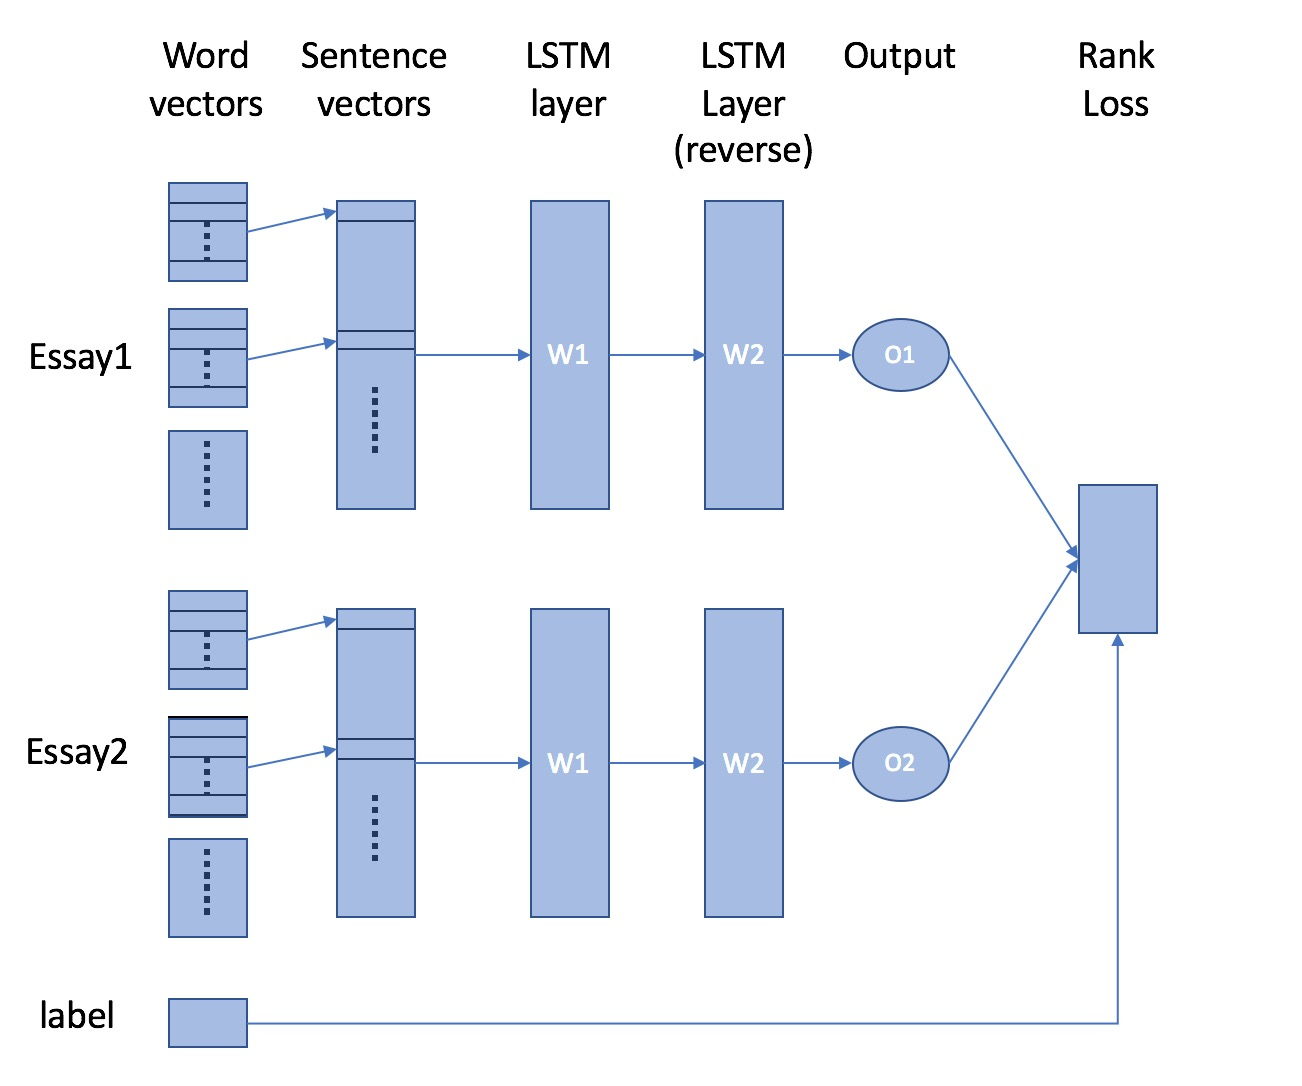
\includegraphics[width=0.6\textwidth]{rankmodel.jpg}
	\caption{Architecture of sentence-level LSTM model with pairwise ranking loss. Note that the weights of the two LSTM models are shared.}
	\label{fig:rankmodel}
\end{figure}

\subsection*{Passage-Level Bidirectional LSTM Model}\hfill\\
\vskip -0.1in

Finally, we consider a passage-level model that is designed to take into account as much information regarding the structure of an essay as possible. The wording, ordering of words, sentence structure, sentence length and essay length are all encoded naturally in this model. The model is constructed as follows, with the architecture depicted in Figure \ref{fig:bilstm}.

For each essay, all sentences is padded with START and END tokens. All of the words, including START and END, are encoded as an integer index, and misspelled words or words with low frequency are denoted as 0. All essays are padded into fixed length sequence of integer indices. Short essays are padded with 0 and long essays are truncated from the end. The sequences of indices representing each essay are transformed into sequences of vectors using pretrained GloVe embedding with dimension of 300. These sequences of word embeddings are then fed into a bidirectional LSTM model, which yields passage-level vector representations. The passage-level encoded vectors, i.e. the last outputs of this bidirectional LSTM model, are concatenated together (forward and reverse direction) and fed into the output layer. As with the word-level models, the output layer could either be a softmax with 61 units or one unit with linear activation, for classification and regression respectively.

\begin{figure}
	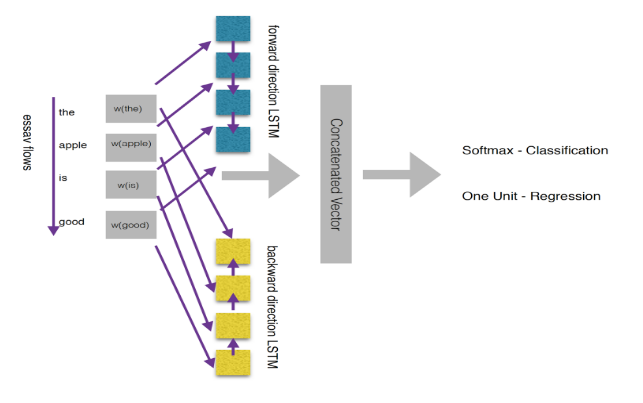
\includegraphics[width=0.6\textwidth]{bilstm.png}
	\caption{Architecture of passage-level bidirectional LSTM model using either softmax output for classification or linear output for regression.}
	\label{fig:bilstm}
\end{figure}

\section*{Metrics}

For the purposes of investigating the respective strengths of the various models considered above, we also consider a number of different evaluation metrics, which highlight different performance properties. We note that these are {\em not} the metrics used during training, but rather metrics used to evaluate the performance of the models on the test set. For all formulas, we let $p_i$ to be the predicted score on the essay $i$ and $y_i$ to be the actual score, with a total test size of $N$.

\subsection*{Classification Accuracy}

As the essay grading problem is often treated as a classification problem (each discrete score being a ``category'' of essays), we consider evaluating on the simplest classification metric, namely that of accuracy on the test set:
$$ACC \equiv \frac{1}{N} \sum_{i=1}^N \mathbb{I}_{p_i = y_i}$$
where $\mathbb{I}_{x=y}$ is an indicator of whether $x=y$.

\subsection*{Mean-Squared Error (MSE)}

One issue with a raw classification accuracy metric is that it does not provide any indication of the discrepancy between the actual and predicted scores. For example, on a scale of 2-12, a model predicting a score of 3 would incur the same loss as a model predicting 9 for an actual score of 10. We would clearly prefer the latter model over the former model, however; indeed, for grading purposes, it is not as important to achieve the exact same score so much as it is to obtain predictions that are on average close to the actual scores.

Thus, we consider the traditional mean-squared error (MSE) as one of our metrics, namely:
$$MSE \equiv \frac{1}{N} \sum_{i=1}^N (p_i - y_i)^2$$

\subsection*{Normalized Discounted Cumulative Gain (NDCG)}

In addition to the classification accuracy and MSE, we also report NDCG to measure the ranking quality of a model. In our problem, each essay has a discrete score that can be compared with the scores of other essays in the same essay set, while scores of essays from different essay sets are not comparable since the score range of essay sets are different. For each essay set, we compute the Discounted Cumulative Gain (DCG):
 
$$DCG=\sum_{i=1}^n\frac{score_i}{log_2(i+1)}$$
where $score_i$ is the score of essay that is ranked at the \textit{i}th position among all essays from the same essay set by the model. The premise of DCG is that essay with high score but ranked lower by the model should be penalized, as the score is reduced logarithmically proportional to the rank given by the model.

In our problem, essay sets contain different number of essays, hence comparing a model's performance from one essay set to the other cannot be consistently achieved using DCG alone. To address this issue, we report the Normalized Discounted Cumulative Gain (NDCG) instead:

$$NDCG=\frac{DCG}{IDCG}$$
where IDCG(Ideal DCG) is the maximum possible DCG obtained by sorting all essays in the set by their scores and then calculating the DCG.

\subsection*{Quadratic Averaged Kappa}
Another metric we considered is Quadratic Averaged Kappa, which measured the degree of agreement between two raters and weighted over the distance between different categories. For example, a score of 5 will gain more penalty if it is predicted as 8 than it is predicted as 6. The range of Quadratic Averaged Kappa is from -1 to 1, and 1 implies perfect agreement while 0 implies a random guess. 

To calculate the Quadratic Averaged Kappa, one need to construct two N by N matrix $O$ and $E$, where N is the number of different grades. $O_{i,j}$ corresponds to the number of essays that received a rating i by Rater A and a rating j by Rater B. Therefore, the summation of $O$ across all i and j should be the total number of essay. For the matrix $E$, we first obtain two length-N vector $u$, $v$, where $u_i$ and $v_i$ represent the number of essay receiving a rating i from rater A and rater B respectively. The matrix $E$ is then the outer-product of vector $u$ and $v$, such that $O_{i,j} = u_i v_j$. Then the matrix $E$ is normalized so that it has same sum as the matrix $O$.

Another weight matrix $W$ is calcaluated as following:
$$
W_{i,j} = \frac{(1-j)^2}{(N-1)^2}
$$

Finally the Quadratic Averaged Kappa is calculated:
$$
k = 1 - \frac{\sum_{i,j}w_{i,j}O_{i,j}}{\sum_{i,j}w_{i,j}E_{i,j}}
$$




\section*{Results and Discussion}

Our results are presented in Table \ref{fig:eval}, with the hyperparameter and architectural settings determined on validation given in Table \ref{fig:params}. Most importantly, we find that deep networks with a variety of architectures can perform competitively with the results of the models from the 2012 competition, which generally employed painstakingly hand-crafted features that do not generalize across essay prompts.

Another result to note not properly reflected in the tables is that our models were often able to distinguish between the different essay prompts with no explicit guidance. In other words, the models automatically classified or predicted scores that fell into the proper score range for each test essay without needed other information regarding the essay set. As such information was provided explicitly to previous models, this demonstrates the learning capacity of deep architectures to both perform well on this task as well as to generalize information across prompts.

Finally, we find that different architectures provide different strengths in terms of final performance on the test set. For example, the character-level CNN models were able to perform quite well on classification accuracy and RMSE, but generally failed to perform as well on the quadratic kappa or nDCG metrics. This indicates that character-level CNN models obtain good predictions for many essays, but that on similarly-scored essays may fail to resolve these scores into the proper ranking. On the other hand, models that captured sequential information such as the sentence- or passage-level LSTMs performed very well on the nDCG and quadratic kappa metrics, indicating that even when these models failed at predicting precisely the right score, they often were able to predict scores that were close to the actual ones and ranked essays properly. These results suggest that depending on the preferences of the assessor, different models for essay grading may be more suitable.


\begin{table}
	\begin{tabular}{c|c|c|c|c}
		Model & Accuracy & MSE & nDCG & Quad. Kappa \\\hline
		Char-level CNN (1-layer, one-hot) & 68.3\% & 0.782 & 0.923 \\
		Char-level CNN (1-layer, embed) & 66.7\% & 1.158& 0.910\\
		Char-level CNN (6-layer, one-hot) & 38.9\% & 1.039 & 0.929 \\
		Char-level CNN (6-layer, embed) & 36.7\%& 1.179 & 0.910 \\
		Word-level DNN Classification (5-layer,GloVe embed) & & &  \\
		Word-level DNN Regression(5-layer, GloVe embed) & & &  \\
		Sentence-level LSTM & -- & -- & 0.9482 \\
		Passage-level Bi-directional LSTM Classification (GloVe embed) & & &  \\
		Passage-level Bi-directional LSTM Regression(GloVe embed) & & & 
		
	\end{tabular}
	\caption{Performance on test set evaluated via the metrics discussed above.}
	\label{fig:eval}
\end{table}


\begin{table}
	\begin{tabular}{c|c|c|c|c|c}
		Model & Embed Dim. & Filter Sizes & Num. Filters & Pooling & Hidden Dim. \\\hline
		Char-level CNN (1-layer, one-hot) & -- & 64 & 64 & 64 & 32 \\
		Char-level CNN (1-layer, embed) &  30 & 64 & 128 & 64 & 32 \\
		Char-level CNN (6-layer, one-hot) & -- & $(64, 32, 16, 8, 4, 2)$ & 64 & $(4,4,4)$ & 64 \\
		Char-level CNN (6-layer, embed) & 30 & $(64, 64, 32, 16, 4, 4)$ & 64 & $(6,4,4)$ & 128 \\
		Word-level MLP  & & & & & \\
		Word-level LSTM  & & & & & \\
		Word-level Bi-LSTM  & & & & & \\
		Ranking Model & & & & & \\
		...  & & & & &
	\end{tabular}
	\caption{Hyperparameter and architectural choices as selected by performance on validation. Hyperparameter settings that are irrelevant for certain models are omitted (--).}
	\label{fig:params}
\end{table}


\section*{Member Contributions}

\subsection*{Won Lee}

Prior to the switch in our project from music-to-lyric generation to automated essay grading, I conducted all data generation (i.e. cleaning, formatting, compiling music-lyric pairs, etc.) and finalized models and training for training/evaluation on Harvard's clusters. With regard to essay grading, I developed all of the character-level and CNN-based models and conducted exhaustive grid search and training for these models for both classification and regression tasks. I also contributed to the evaluation script (MSE, accuracy, etc.) as well as various data-related auxiliary scripts for loading onto the models. Finally, I did most of the write-up for the current report as well as the proposal, and standardized output/formatting for the scripts and informative files.

\subsection*{Qin Lyu}

Prior to the switch, I designed the NN-based model and intensively explored its ability for music-lyric generation. With regard to essay grading, I developed all of the sentence-level LSTM models, and proposed to use the pairwise ranking loss to model the order information, and also proposed to use NDCG as an alternative measure of grading quality. I also contributed to the evaluation script (NDCG part) as well as data preprocessing script.

\subsection*{Zelong Qiu}
During the first stage before switch to current project, I wrote the script of pre-processing data and concatenating music and lyric into batches of pairs. I also built and tested a baseline model using similarity search. After switch to automatic essay grading, I did the following four parts: 1) wrote the script of processing raw data into rational table and splitting the train/validate/test for model building; 2) wrote the of evaluation script for quadratic averaged kappa; 3) developed and tested the word-level DNN models (classification/regression), as well as the passage-level bi-LSTM models (classfification/regression). 4) contributed to the corresponding parts in the final report. Designed the layout of presentation poster and completed corresponding parts of it.

\begin{thebibliography}{99}
\bibitem{iea}
Foltz, P. W., et al. (2013). ``Implementation and applications of the Intelligent Essay Assessor.'' {\em Handbook of Automated Essay Evaluation}: 68-88.

\bibitem{erater}
Attali, Y. and J. Burstein (2006). ``Automated Essay Scoring with e-Rater V2.'' {\em The Journal of Technology, Learning and Assessment} 4.

\bibitem{collobert}
Collobert, R.

\bibitem{glove}
Jeffrey Pennington, Richard Socher, and Christopher D. Manning. 2014. GloVe: Global Vectors for Word Representation.

\bibitem{ranknet}
Burges, C., Shaked, T., Renshaw, E., Lazier, A., Deeds, M., Hamilton, N., and Hullender, G. (2005). Learning to rank using gradient descent. In Proceedings of the 22nd international conference on Machine learning (pp. 89-96). ACM.


\end{thebibliography}

\end{document}